\documentclass[12pt,a4j,twoside]{jarticle}

\usepackage{gradthesis}
\usepackage{amsmath}
\usepackage[dvipdfmx]{graphicx}
\usepackage{amssymb}
\usepackage{color}
\usepackage{algorithm}
\usepackage{algorithmic}

\newcommand{\argmax}{\mathop{\rm arg~max}\limits}
\newcommand{\argmin}{\mathop{\rm arg~min}\limits}
\def\AgentSet{A}
\def\Dreq{{D_{\it req}}}
\def\En{\mathcal{E}}
\def\SelfAss{{S_{\it ass}}}

\def\BatteryMax{{B_{\it max}}}
\def\BatteryLevel{b}

\def\HomingCheck{{T_{\it homing}}}
\def\HomingBattery{{k_{\it homing}}}
\def\PausingInt{{S_{\it pause}}}

\def\PauseTimeFactor{{\gamma_{\it p}}}

\def\DeactCheckStartTime{D_{\it st}}
\def\DeactCheckInterval{D_{\it int}}
\def\PauseCount{x_{\it pause}}
\def\DeactCount{N_{\it deact}}
\def\DeactThreshold{K_{\it deact}}



\def\green#1{\textcolor[rgb]{0,0.6,0}{#1}}
\def\dgreen#1{\textcolor[rgb]{0.02,0.50,0.05}{#1}}
\def\gray#1{\textcolor[rgb]{0.5,0.5,0.7}{#1}}
\def\red#1{\textcolor{red}{#1}}
\def\blue#1{\textcolor{blue}{#1}}
\def\Blue{\color[rgb]{0,0,1}}
\def\Red{\color[rgb]{1,0,0}}
\def\Dgreen{\color[rgb]{0.02,0.55,0.04}}
\def\Black{\color[rgb]{0,0,0}}
\def\ignore#1{}
\def\original#1{}

\title{マルチエージェント協調巡回問題におけるエネルギー消費抑制手法の提案}{5}
\etitle{hoge}
\author{松本~航平}
\studentid{1W193102}
\university{早稲田大学}
\faculty{基幹理工学部}
\department{情報理工学科}
\type{卒業論文}
\nendo{2022}
\hizuke{2023/}
\advisor{菅原~俊治}

\begin{document}
\maketitle

\begin{abstract}
  \red{後で追記する}
  \par
  
\end{abstract}

\vspace*{1cm}\par
\section{序論}
\label{sec:introduction}
\red{後で追記する}
\par

近年,ロボット技術が発達し,巡回パトロールや清掃などといった,人間が日常的に繰り返す作業や,
災害地や原子力発電所,宇宙などでの作業を複数の自律的ロボットで代替する動きが加速している.
このような複数のロボットが協調して共通の作業を行う問題は,ロボットを自律的に動作するエージェントとしてモデル化し,
マルチエージェント協調巡回問題({\em multi-agent cooperative patrolling problem}, MACPP)と呼ばれる.
MACPPの研究では,複数のエージェントが協力・協調することで,
与えられた環境において効率的かつ効果的に巡回を行うための方法・アルゴリズムを見出すことを目的としている.
\par

巡回効率だけを追求した高度な行動や学習は,確かに巡回の効率は向上するものの,
必要以上にエネルギーを消費する可能性があり,これはMACPPの極めて大きな課題となっている.
特に,本研究で想定する自律型エージェントは独自のバッテリを持ち,頻繁な充電を強いられることになる.
一方,アプリケーションによっては,巡回作業に対する品質要求があり,
それを超えることは必ずしも期待されているわけではない.
例えば,清掃問題では,ある程度環境がきれいになっていれば十分であり,
過度の巡回作業はかえって単位エネルギー当たりの作業効率を低下させる.
また,環境が複雑で大規模な場合,どれだけのエージェントが必要かを事前に判断することができないこともあり,
エージェントが少ないと品質要求を満たせず,多すぎるとエネルギーの浪費に繋がる.
\par

マルチエージェントシステムにおける協調の観点からエネルギー効率に注目した研究\cite{Kim2016,Benkrid2019,Notomista2022}がある.
例えば,\cite{Benkrid2019}では,マルチロボットにおける探索問題において,
移動ロボットの総運動エネルギーを節約するために,運動時間を短縮する分散型協調手法を提案している.
しかし,これらの研究は,タスクのために効率的に移動・作業し,
結果として総消費エネルギーを削減する方法を目指したものである.
一方,本手法では,他のエージェントが要求されるタスクの質を満たすことができれば,
あるエージェントが自らの判断でしばらく停止したり,システムから退出したりすることを実現しようとするものである.
また,\cite{WuPrima2019, Wu2019}では,エージェントが要求を満たせば自律的に一時停止してエネルギーを節約し,
再び充電して探索に戻るという手法を提案している,
しかし,その方法は不十分であり,エージェントは依然として不必要に環境内を巡回していることが分かった.
\par

そこで本研究では,\cite{Wu2019}の手法を拡張し,その後の行動によって起こりうる貢献を自律的に予測し,
環境の現状を推定することで要求品質の全体的な達成度を把握しながら,
より効率的に要求品質の充足とエネルギー消費の削減を両立する手法を提案する.
主な違いは,エージェントが休止・充電している間の巡回タスクの進捗は,
他のエージェントの行動に依存し,エージェントごとに異なるため,
個々のエージェントから見たエネルギー節約行動の自律学習を導入しているという点である.
\par

さらに,この学習が進むとエージェントは,短い休止時間で巡回するBusyグループと,
比較的長い時間休止してエネルギーを消費しないEnergy saveグループに分かれることを発見した.
そのため,後者のグループのエージェントは,品質要求を満たしたまま,順次,活動を停止することができる,
実験の結果,提案手法により,従来手法と比べて大幅にエネルギー消費量を削減することができることが分かった.
また,Busyグループに属するエージェントの数は,環境条件によって変化することが分かった.
その後,品質要求を満たしつつ,Energy saveグループに属するエージェントを順次停止することで,
活動しているエージェント数を削減することができた.
\par

\section{関連研究}
\red{後で,杉山さんの研究も追加する、領域分解についても追加(SMASH参考)}

MACPPとその応用に関する研究は数多く行われている\cite{Hattori2021,Tevyashov2022,Wiandt2018,Othmani2017,Zhou2019}.
例えば, \cite{Othmani2017}では,{\em edge Markov evolution graphs}を用いた動的環境変化のモデルを提案した.
また,\cite{Zhou2019}では,巡回問題をベイズ適応型遷移分離部分観測可能マルコフ決定過程として定式化し,
モンテカルロ木探索法を拡張した分散型オンライン学習・計画アルゴリズムを提案している.
さらに,\cite{Othmani2018}では,人口ニューラルネットワークを用いて,
個人のidlnessから共用のidlnessを予測する方法を提案している.
しかし,これらの研究では,バッテリの放電やエネルギー消費による定期的な充電を無視し,
効率性のみを考慮したものである.
\cite{Yoneda2013}では,Q学習によって決定される計画戦略のもと,
複数のエージェントが定期的に充電しながら協調して巡回するAMTDS({\em adaptive meta-target decision strategy})という手法を提案している.
さらに,\red{ここから杉山さんの研究}.
しかし,この研究もエネルギー消費量の削減を考慮せず,巡回の効率化を目的とした学習のみを行うものである.
\par

一方,\cite{Kim2016,Benkrid2019,Notomista2022,Kim2016,Wu2019,Latif2021}では一部,省エネルギーに着目している.
\cite{Kim2016}では,消防ロボット以外にも複数のサブロボットを導入し,消火作業における総作業時間の延長を図った.
また,\cite{Latif2021}では,協調型群ロボットに対して,
採餌などの連続タスクを解決するためのエネルギー配慮型分散タスク配分アルゴリズムを提案し,
高効率なミッションの実現を実現した.
しかし,これらの研究では,本研究とは異なり,動作時間の延長も考慮されている.
これに対して,\cite{Wu2019}では,AMTDSを巡回の品質要求に合わせて拡張し,省エネルギー化を図った.
しかし,この手法によるエネルギー削減は不十分であり,エージェントの活動にはまだ不要な行動が含まれている.
そこで,本研究では,個々の視点からの学習を導入することで,品質要求を満たしながら,さらにエネルギー消費を削減した.
さらに,複数のエージェントを停止する手法を提案し,消費エネルギーの削減を図った.

\section{モデルの定義}
\label{sec:MACPP_model}
本研究は,\cite{Wu2019}で提案された清掃問題におけるエネルギー節約手法である,
{\em adaptive meta-target decision strategy for energy saving and cleanliness} (AMTDS/ESC)
の拡張である.
また,従来手法との比較を行うため,本研究で用いる問題の定式化と環境,エージェントの活動モデルは
\cite{Wu2019}で用いられているものを踏襲する.
\par

\subsection{環境}
エージェントの巡回環境を,2次元ユークリッド空間に埋め込み可能なグラフ$G = (V,E)$で表す.
ここで,$V = \{v_1, \dots, v_n \}$はノード集合を表し,
各ノード乗にエージェントやイベント,障害物が存在する.
また,$E$はエージェントが移動する経路に対応するノード$v_i$と$v_j$間のエッジ$e_{i,j}$である.
\par

さらに,ステップを単位とする離散時間を導入する.
簡単のため,必要に応じてダミーノードを追加することで,全てのエッジの長さは1に保たれる.
したがって,エージェントは1ステップで障害物のない隣接ノードに移動することができる.
ここで,$v_i$と$v_j$の最短距離(エッジの数)を$d(v_i,v_j)$とする.
\par

全てのノード$v\in V$上でイベントが発生し,そのイベント発生確率を$p(v)~(0\leq p(v)\leq 1)$とする.
毎時刻$t$において,ノード$v$に蓄積されたイベント数$L_t(v)$は以下の式で更新される.
%
\[
L_t(v) = \left\{
\begin{array}{ll}
  L_{t-1}(v) + 1 & \textrm{(確率$p(v)$のイベント発生時)} \\
  L_{t-1}(v) & \textrm{(その他)}
\end{array}
\right.
\]
%
時刻$t$にエージェントがノード$v$を訪れた時に$v$上のイベントは処理され,$L_t(v) = 0$となる.
イベントの解釈は,アプリケーションによって異なり,例えば,掃除のアプリケーションでは,
$p(v)$は場所$v$の汚れやすさを,$L_t(v)$は汚れの蓄積度合いを表す.
また,防犯監視パトロールのアプリケーションでは,$p(v)$はアプリケーションの所有者が指定した,
重要な場所に対する必要な防犯度合いを示し,$L_t(v)$は警戒レベルと解釈することができる.
本研究では,全ノードの$p(v)$はあらかじめ指定されていると仮定する.

\subsection{エージェント}
$n$個のエージェントの集合を$\AgentSet=\{1,\dots ,n\}$と表す.
エージェント$i\in\AgentSet$はバッテリを持ち,充電基地$v^i_{base}$で充電を繰り返すことで連続動作が可能である.
つまり,バッテリが満タンの状態で$v^i_{base}i$を出発した$i$は,環境を巡回し,
再び$v^i_{base}$に戻ってくるという動作をする.
エージェント$i$のバッテリ性能を$(B^i_{max}, B^i_{drain}, k^i_{charge})$で表す.
ここで,$B^i_{max}$はエージェントのバッテリ容量,$B^i_{drain}$は1ステップで消費するバッテリ消費量,
$k^i_{charge}$はバッテリ残量を1増加させるために必要なステップ数である.
時刻$t$におけるエージェント$i$のバッテリ残量を$\BatteryLevel_i (0 \leq \BatteryLevel_i \leq B_{max})$とすると,
$i$が1ステップで隣接するノードに移動したとき,$\BatteryLevel_i(t)$は以下の式に従って更新される.
%
\begin{equation}
  \BatteryLevel_i(t+1) \gets \BatteryLevel_i(t) - B^i_{drain}
\end{equation}
%
\par

$b^i(t)$が0になるとそのエージェントは移動できなくなってしまうので,自身のバッテリ残量が0になる前に戻らなければならない.
そこで,以下の式に示すように,エージェント$i$はノード$v$から充電基地$v^i_{base}$までの移動に必要な最小バッテリ量であるポテンシャル$\mathcal{P}^i(v)$を計算する.
%
\begin{equation}
  \mathcal{P}^i(v) = d(v, v^i_{base}) \times B^i_{drain}
\end{equation}
%
エージェント$i$は目標ノード$v^i_{tar}$を後の章で説明する目標決定戦略によって決定した際,実際に移動する前に,
現在のバッテリ残量で$v^i_{tar}$に到達し,その後充電基地に戻ることができるかを,以下の式を用いて判定する.
%
\begin{equation}
  b^i(t) \leq \mathcal{P}^i(v) + d(v^i_t, v^i_{tar}) \times B^i_{drain}
\end{equation}
%
この条件を満たさない場合,以下のように目標ノード$v^i_{tar}$を更新し,充電基地に戻る.
%
\begin{equation}
  v^i_{tar} \gets v^i_{base}
\end{equation}
%
エージェントは$v^i_{base}$に到着後,バッテリ残量が最大になるまで充電し,充電完了後は再び環境を巡回する.
ここで,満充電(つまり,$\BatteryLevel_i=\BatteryMax$)になるまでに,
$(\BatteryMax-\BatteryLevel_i)\times k_{charge}$ステップかかる.
\par

エージェント$i$は,すべてのノード$v$に対し,$v$のイベント発生確率の予測値を表す重要度$p^i(v) (0 \leq p^i(v) \leq 1)$を持つ.
$p^i(v)$は各エージェントが独立して保持しており,その値はエージェントごとに異なる.
$i$が$v$上にいない場合,現在の蓄積イベント数$L_t(v)$は知ることができない.
そこで,エージェントは時刻$t$の$p(v)$から期待値$E^i(L_t(v))$を以下の式に従って計算する.
%
\begin{equation}
  E^i(L_t(v)) = p^i(v) \times (t - t^v_{vis})
\end{equation}
%
この計算のために,エージェントは自分と他のエージェントの位置を知ることができると仮定する.
これは,現在の技術で容易に実現可能であるためである.
例えば,赤外線やGPSなどのセンサーを用いたり,エージェント間で直接通信したり,
クラウドロボティクス,すなわち,クラウドを介して情報を共有したりすることで実現できる.
しかし,エージェントは目的地を設定するための戦略や,目的地までの計画経路など,
エージェント内部の情報や判断を共有・推論することはできない.
\par

また,エージェント$i$と$j$はエージェント間の情報交換や交渉を用いる際に,互いに通信可能である.
しかし,エージェントの過度の通信によるコスト増加や干渉を防ぐために,通信可能範囲$d_{co}(>0)$が存在する.
$i$と$j$が以下の式を満たすとき,互いに通信可能である.
%
\begin{equation}
  m(v^i, v^j) < d_{co}
\end{equation}
%
加えて,同様の目的から,時間面の制約である最低通信間隔$B(>0)$が存在する.
$i$は$j$と最後に通信した時刻$T^{i, j}_{lst}$を保持しており,$T^{i, j}_{lst} + B$まで通信を行うことはできない.
\par

さらに,本研究では,要求品質を満たしつつエネルギー節約行動を学習することに重点を置いており,
実験で用いたグリッド状の環境では,衝突を回避する迂回経路の生成が容易であると考えられるため,
エージェント間の衝突は考慮しないこととする.
\cite{Yamauchi2022,Satish2017}のように,衝突が発生しない経路を生成するアルゴリズムはいくつか提案されており,
これらのアルゴリズムの1つを衝突回避に用いることができる.

\subsection{評価指標}
評価指標は,扱うMACPPの種類によって異なるが,本研究では評価指標として,
以下の式で定められるイベント残存時間の総和$D_{t_s,t_e}$と,エージェントの総エネルギー消費量$C_{t_s,t_e}$を用いる.
%
\begin{align}
  D_{t_s,t_e} &= \sum_{v \in V} \sum^{t_e}_{t=t_s+1} L_t(v)\\
  C_{t_s,t_e} &= \sum_{i \in \AgentSet} \sum^{t_e}_{t=t_s+1} \En_t(i),
\end{align}
%
ここで,$[t_s,t_e]~(t_s < t_e)$ は時間間隔を表し,
$\En_t(i)$は$t$におけるエージェント$i$の消費エネルギーを表す.
したがって,$i$が隣接ノードに移動したとき$\En_t(i)=1$,
それ以外は$\En_t(i)=0$となる.
例えば,$D_{t_s,t_e}$は清掃問題において,掃除機をかけずに放置した埃の累積時間や,
セキュリティパトロールにおいて,チェックせずに放置したセキュリティ場所の累積時間や数を表し,
MACPPではこれを減らすことが目的となる.
\par
一般に,$D_{t_s,t_e}$と$C_{t_s,t_e}$の値はどちらも小さい方が良いとされるが,両者はトレードオフの関係である.
つまり,$D_{t_s,t_e}$と$C_{t_s,t_e}$の値をどちらも最小にすることは困難である.
したがって,\cite{Wu2019}と同様に1stepにおけるイベント量の要求値$\Dreq$を設定した.
エージェントは以下の式を満たせるように協調を行う.
%
\begin{equation}\label{eq:condition}
  D_{t_s,t_e}\leq \Dreq \times (t_e - t_s)
\end{equation}
%
本研究では,品質要求(式(\ref{eq:condition}))を満たしつつ,$C_{t_s, t_e}$をできるだけ小さくすることが目的である.
なお,本研究では単純化のため,これ以降,$D_{t_s,t_e}, C_{t_s,t_e}$を$D(s), C(s)$と表す.

\section{準備}
この章では,提案手法の基になったAMTDS,AMTDS/LD,AMTDS/EDC,AMTDS/ESCについて説明する.
これらの手法では,エージェントは目標ノード$v^i_{tar}$を決定する目標決定戦略と,それまでの経路を生成する経路生成戦略に従い,環境内を巡回する.
$v^i_{tar}$に到着した後,再び目標戦略に従って新しい目標ノードを決定するといったサイクルを各エージェントが繰り返し,継続的な環境巡回を行う.

\subsection{Adaptive meta target decision strategy (AMTDS)}
\label{subsec:AMTDS}
この節では,AMTDS/LD,AMTDS/ESCなどの手法のベースとなったAdaptive meta target decision strategy (AMTDS) \cite{Yoneda2013}について説明する.
AMTDSは単純な複数の目標決定戦略の中から,強化学習アルゴリズムであるQ学習によって,各エージェントが自身にとって最適な戦略を選択するメタ戦略学習である.
また,この手法では環境内のすべてのノード$v$におけるイベント発生確率$p(v)$は既知であるという仮定を導入しており,$p^i(v) = p(v)$とする.
\par

エージェント$i$はAMTDSによって目標決定戦略$s \in S$を選択し,$s$に従って目標ノード$v^i_{tar}$を決定する.
その後,経路生成戦略に従って$v^i_{tar}$に移動する.
ここで,$S$はエージェントが選択可能な目標決定戦略の集合である.
目標決定戦略については\ref{target_strategy},経路生成戦略については\ref{route_strategy}で詳細を説明する.
$v^i_{tar}$に到着後,$v^i_{tar}$の決定時刻$t_0$から$d_{travel}$ステップ後に$v^i_{tar}$に到着するまでの1ステップあたりのイベント処理量を以下の式で計算する.
%
\begin{equation}
  \label{eq:reward_AMTDS}
  u_{t_0,t_0+d_{travel}} = \dfrac{\displaystyle\sum_{t_0+1 \leq t \leq t_0+d_{travel}} L_t(v^i_t)}{d_{travel}}
\end{equation}
%
さらに,これを報酬として,選択した戦略$s$のQ値$Q^i(s)$を以下の式に従って更新する.
%
\begin{equation}
  Q^i(s) \gets (1-\alpha)Q^i(s) + \alpha \times u_{t_0,t_0+d_{travel}}
\end{equation}
%
ここで,$\alpha (0 < \alpha \leq 1)$は学習率である.
$Q^i(s)$の更新後,$i$は次に選択する目標決定戦略$s_{next}$を$\varepsilon$-Greedy法によって決定する.
$\varepsilon$-Greedy法では,$s_{next}$を確率$\varepsilon$でランダムに選択し,確率$1 - \varepsilon$で以下の式に従って選択する.
%
\begin{equation}
  s_{next} \gets \argmax_{s} Q^i(s)
\end{equation}
%

\subsubsection{目標決定戦略}
\label{target_strategy}
\cite{Yoneda2013}では,各エージェントに以下の4つの基本的な目標決定戦略を$S$として与えている.
それぞれの戦略は単独でも使用可能な独立したものとなっている.
単独での使用を想定し,競合回避のためにランダム性を取り入れたものも存在する.
%
\begin{description}
  \item[Random selection (R)]\mbox{}\\
  環境全体のノード集合$V$からランダムに$v^i_{tar}$を選ぶ.

  \item[Probabilistic greedy selection (PGS)]\mbox{} \\
  環境全体のノード集合$V$内のノード$v$におけるイベント発生量の推定値$E^i(L_t(v))$の上位$N_g$個のノードから,
  ランダムに1つ$v^i_{tar}$を選ぶ.
  この際に,学習や訪問をする$v^i_{tar}$の偏りを防ぐため,$N_g$番目のノードと$E^i(L_t(v))$の値が同じノードが存在する場合,
  そのノードをすべて含めた後,その中から$v^i_{tar}$をランダムに選んでいる.

  \item[Prioritizing unvisited interval (PI)]\mbox{} \\
  環境全体のノード集合$V$内のノード$v$における訪問間隔$I^i_t(v)$の上位$N_i$個のノードから,ランダムに1つ$v^i_{tar}$を選ぶ.
  この際に,学習や訪問をする$v^i_{tar}$の偏りを防ぐため,$N_i$番目のノードと$I^i_t(v)$の値が同じノードが存在する場合,
  そのノードをすべて含めた後,その中から$v^i_{tar}$をランダムに選んでいる.
  
  \item[Balanced neighbor-preferential selection (BNPS)]\mbox{} \\
  近隣のノードにイベント発生量が多いとエージェントが判断したとき,近隣を優先的に巡回する.
  $v^i_{tar}$の決定時にエージェントの現在地$v^i_t$との距離が$d_{rad}$以下のノード集合を近領域$V^i_{area}$とする.
  ここで,$V^i_{area}$における1ステップあたりのイベント処理量の期待値$EV^i_t$は以下の式で求められる.
  \begin{equation}
    EV^i_t = \frac{\displaystyle \sum_{v \in V^i_{area}}E^i(L_t(v))}{|V^i_{area}|}  
  \end{equation}
  エージェント$i$は近領域内のイベントを処理するか判断するための閾値$EV_{threshold}$と$EV^i_t$の値を比較し,
  $EV^i_t > EV_{threshold}$の間はPGSによって近領域内から$v^i_{tar}$を選ぶ.
  その後,$EV^i_t \le EV_{threshold}$となった場合,環境全体を対象とし,PGSで$v^i_{tar}$を選ぶ.
  環境全体から$v^i_{tar}$を選択した後,$V^i_{area}$を更新する.
  更新後の$V^i_{area}$の1ステップあたりのイベント処理量の期待値を$EV^i_{t+1}$とし,
  $EV_{threshold}$の値を以下の式に従って更新する.
  \begin{equation}
    EV_{threshold} \gets EV_{threshold} + \alpha(EV^i_{t+1} - EV_{threshold})
  \end{equation}
  ここで,$\alpha(0 < \alpha < 1)$は学習率である.
  また,$EV_{threshold}$の初期値は初めに$V^i_{area}$を設定した際の$EV^i_t$の値である.
\end{description}
%

\subsubsection{経路生成戦略}
  \label{route_strategy}
  経路生成戦略は{\em gradual path generation} (GPG)を用いる.
  GPGでは,まず$v^i_{tar}$までの最短経路をダイクストラ法を用いて生成し,
  その経路近辺でイベントが発生しやすいノードを経由するように経路を変更する.
  これにより,最短経路に従うよりも効率を高めることができる.
  しかし,経由するノードの増加によって$v^i_{tar}$への到着時間が遅れてしまい,逆に効率が下がってしまう.
  そのため,経由するノードに一定の制約をかけなければならない.
  そこで,GPGでは経由可能なノード$v$を以下の式を満たすものとする.
  %
  \begin{equation}
    \begin{cases}
      d(v^i_t, v) \leq d_{myopia} \\
      d(v, v^i_{tar}) < k_{att}(d(v^i_t, v^i_{tar})) \\
      d(v^i_t, v) + d(v, v^i_{tar}) \leq k_{rover}d(v^i_t, v^i_{tar}) \\
      \mathcal{P}^i(v^i_{tar}) + B^i_{drain} \times (d(v^i_t, v) + d(v, v^i_{tar})) \leq b^i(t)
    \end{cases}
  \end{equation}
  %
  ここで,$d_{myopia}$はエージェントが現在地とするノードから経由地点とできるノードまでの距離の閾値であり,
  $k_{att} (0 < k_{att} < 1)$は$v^i_{tar}$へ引き付ける力を表す係数である.
  また,$k_{rover} (1 < k_{rover})$は経由地点を追加した新しい経路の距離の,最短距離からの増加率である.
  これらの条件を満たすノード集合を$V^i_{sub}$とすると,経由するノード$v^i_{subgoal}$は以下の式で決められる.
  %
  \begin{equation}
    v^i_{subgoal} \gets \argmax_{v \in V^i_{sub}} E^i(L_t(v))
  \end{equation}
  %

  \subsection{AMTDS with learning of dirt accumulation (AMTDS/LD)}
  \label{subsec:AMTDS/LD}
  AMTDSでは,エージェントが環境内のすべてのノード$v$において,
  イベント発生確率$p(v)$をあらかじめ把握しているという仮定を導入した.
  しかし,実際の利用を想定すると,イベント発生確率が既知であることはまれである.
  特に,本研究のような清掃問題においては,イベントであるごみの発生確率を,
  エージェントが巡回しながら自ら学習するほうがより実用的である.
  そこで,AMTDSに環境のイベント発生確率の学習を加えた,
  AMTDS with learning of dirt accumulation (AMTDS/LD) \cite{Sugiyama2015meta}が提案された.
  AMTDS/LDでは,$p^i(v)$の学習アルゴリズムの提案が行われた.
  以下でこのアルゴリズムについて説明する.
  \par

  まず,1ステップ終わるごとにエージェント$i$はすべてのノードについて,
  そのノードで最後にイベントが処理された時刻$t^v_{vis}$から現在の時刻$t$までの訪問間隔$I^i_t(v)$を以下の式に従って更新する.
  %
  \begin{equation}
    I^i_t(v) = t - t^v_{vis}
  \end{equation}
  %
  その後,$I^i_t(v)$と現在時刻$t$でエージェント$i$が処理したイベント量$L_t(v)$を用いて,
  $i$の$v$における重要度$p^i(v)$を以下の式に従って更新する.
  %
  \begin{equation}
    p^i(v) \gets (1 - \beta)p^i(v) + \beta \dfrac{L_t(v)}{I^i_t(v)}
  \end{equation}
  %
  ここで,$\beta(0 < \beta \leq 1)$は学習率である.
  AMTDS/LDでは各エージェントが独立した$p^i(v)$の値を保持しているため,それに伴い,
  イベント発生量の推定値$E^i(L_t(v))$もそれぞれ異なる.
  また,同じノード上であってもそのノードへの訪問頻度によって,エージェントのイベントの発生しやすさの認識が異なる.
  このことによって,エージェント間の通信を用いずに$p^i(v)$を用いた間接的な分業が可能になる.
  それにより,AMTDSと比べて競合を回避し,効率も向上した.

  \subsection{AMTDS with learning of event probabilities and enhancing divisional cooperation (AMTDS/EDC)}
  \red{後で書く}
  AMTDS/LDでは,エージェント間の交渉を用いずに,$p^i(v)$による間接的なコミュニケーションを用いて,
  エージェント間の分業を促進した.
  しかし,間接的なコミュニケーションでの効率改善には限界があり,エージェントが停止した場合などの環境変化に対応できない.
  そのため,エージェントに責任ノード集合$V^i_R$を導入し,そのサイズを調整するエージェント間の交渉をAMTDS/LDに追加した,
  AMTDS with learning of event probabilities and enhancing divisional cooperation (AMTDS/EDC) \cite{Sugiyama2019}
  が提案された.
  領域分割の手法と大きく異なる点は,AMTDS/EDCでは,エージェントの責任ノードを交渉によって直接決定するのではなく,
  それぞれの環境学習によって,各自が判断する点である.
  このことにより,エージェントの交換する情報が少なくなり,交渉の複雑さを抑制することができる.
  この手法により,環境の変化に対する頑健性を高め,全体の効率をさらに改善した.
  この節では,新たに導入した$V^i_R$と,エージェント間で行う交渉について説明する.
  
  \subsubsection{エージェント間の交渉に用いる情報}
  \label{communicationInformation}
  前述のとおり,AMTDS/EDCでは,エージェント$i$は自身の責任ノード集合$V^i_R(\subset V)$を持ち,
  $V^i_R$はそのエージェントの重要度$p^i(v)$の降順に$N^i_R$個のノード集合と定める.
  $V^i_R$,$N^i_R$の初期値はそれぞれ$V$,$|V|$と定める.
  AMTDSやAMTDS/LDとは異なり,AMTDS/EDCでは,PGSやBNPSを用いて次の目標ノード$v^i_{tar}$を決定する際,
  環境全体のノード集合$V$ではなく,$V^i_R$を用いる。
  これにより,選択対象のノードを減らし,分業をさらに促進することができる.
  エージェントが充電基地に戻るまでの間に,充電基地に戻るまでの環境の学習により,
  $p^i(v)$の値がエージェント間の交渉により$N^i_R$の値が更新されている.
  このため,$i$は充電基地に戻った際,自身の責任ノードの集合$V^i_R$を
  更新された$p^i(v)$,$N^i_R$を用いて再定義する.
  ここで,$p^i(v)$の値が同じノードが複数ある場合,ランダムに並べられる.
  \par

  エージェントは交渉に用いる次の2つの情報を計算する.
  1つは,エージェントの責任ノード集合の重要度の総和$p^i_{sum}$である.
  $p^i_{sum}$の値は以下の式で計算される.
  %
  \begin{equation}
    p^i_{sum} = \sum_{v \in V^i_R} p^i(v)
  \end{equation}
  %
  この値は,責任ノードのイベント発生確率の総和であるため,
  この値が大きいほどそのエージェントはタスクを多く持っているといえる.
  \par

  もう1つは,エージェントの責任ノード集合$V^i_R$の重心$C^i = (x^i_c, y^i_c)$である.
  $C^i$は以下の式で$x^i_c, y^i_c$を計算し,これに最も近いノードを重心ノードと定める.
  %
  \begin{eqnarray}
    x^i_c = \sum_{v \in V^i_R} \dfrac{p^i(v)}{p^i_{sum}}x_v \\
    y^i_c = \sum_{v \in V^i_R} \dfrac{p^i(v)}{p^i_{sum}}y_v
  \end{eqnarray}
  %
  最短距離$d(v_i, v_j)$に関して,$d(C^i, v) < d(C^j, v)$のとき,
  ノード$v$を訪れるコストは,エージェント$i$の方がエージェント$j$よりも小さい,
  つまり,この場合は,$i$が$v$を担当した方が移動のコストが少なく,望ましいといえる.

  \subsubsection{エージェント間の交渉}
  各エージェントは\ref{communicationInformation}で示した情報を用いて,
  エージェント間でNegotiation for Balancing Tasks (公平性のための交渉)と
  Negotiation for Trade-Off of Reaponsibility (改善のための交渉)の
  2種類の交渉を行う.
  エージェント間の交渉は,通信コストの抑制のため,1対1の通信のみとし,
  マネージャーなどを介した複数のエージェント間での交渉は用いない.
  エージェントは以下に述べる2種類の交渉を行うことで,$V^i_R$の改善による性能向上と,
  $p^i(v)$の最適化による分業の促進を図る.
  以下で,2種類の交渉について詳細に説明する.
  %
  \begin{description}
    \item[Negotiation for Balancing Tasks (公平性のための交渉)]\mbox{}\\
      この交渉は,エージェント間のタスクを公平にし,
      一部のエージェントへのタスクの偏りを抑制することを目的としている.
      このため,交渉相手のエージェントよりも自身の重要度の総和が大きい場合,
      自身の担当ノードの重要度の小さいノードの重要度の一部を相手に受け渡す.
      具体的な手段としては,まずエージェント$i$と$j$が以下の式を満たすかを判断する.
      %
      \begin{equation}
        1 + T_c < \dfrac{P^i_{sum}}{p^j_{sum}}
      \end{equation}
      %
      この式を満たした場合,$i$と$j$は公平性のための交渉を行う.
      ここで,$T_c(0 < T_c \ll 1)$はエージェント間のタスクの差の閾値である.
      $i$は,$i$よりも$j$の方が距離が近いノードを$p^i(v)$の降順に並べた
      ノード集合$V^{i, j}_R$を以下の式で定義する.
      %
      \begin{equation}
        V^{i, j}_R = {v \in V^i_R|d(C^i, v) > d(C^j, v)}  
      \end{equation}
      %
      $i$は$V^{i, j}_R$から,$p^i(v)$の小さい$e_g$個のノードにおいて,
      以下の式に従って$i$の重要度の一部を$j$に受け渡す.
      %
      \begin{eqnarray}
        p^j(v) \gets p^j(v) + p^i(v) \times \delta \\
        p^i(v) \gets p^i(v) \times \delta
      \end{eqnarray}
      %
      ここで,$\delta(0 < \delta < 1)$は重要度を受け渡す割合である.
      また,$i$から$j$に受け渡す個数を表す$e_g$を,以下の式に従って求める.
      %
      \begin{equation}
        e_g = \min(N^{i, j}_R - 1, N^i_{gmax}, \lfloor \dfrac{p^i_{sum}}{p^j_{sum}} \times \gamma \rfloor)
      \end{equation}
      %
      ここで,$N^i_{gmax}(0 < N^i_{gmax} < N^i_R)$は,
      急激な変化を抑制するための受け渡すノード数の上限であり,
      $\gamma$は受け渡すノード数を調整するためのパラメータである.
      重要度の受け渡し後,$i$と$j$のノード集合のサイズ$N^i_R$,$N^j_R$を以下の式に従って更新する.
      %
      \begin{eqnarray}
        N^i_R \gets N^i_R - e_g \\
        N^j_R \gets \min(|V|, N^j_R+e_g)
      \end{eqnarray}
      %

    \item[Negotiation for Trade-Off of Reaponsibility (改善のための交渉)]\mbox{}\\
      この交渉は,エージェントのタスクを交換し,
      全体への影響を抑えながらエージェントの巡回コストを減らし,
      全体の効率を高めることを目的としている.
      このため,自身とほぼ同じ重要度を持つエージェントに対し,
      自身よりも移動距離が短いノードをお互いに受け渡す.
      具体的な手順としては,まずエージェント$i$と$j$が以下の式を満たすかを判断する.
      %
      \begin{equation}
        1 - T_c < \dfrac{p^i_{sum}}{p^j_{sum}} < 1 + T_c
      \end{equation}
      %
      この式を満たした場合,$i$と$j$は改善のための交渉を行う,
      ここで,$T_c(0 < T_C \ll 1)$はエージェント間のタスクの差の基準値である.
      $i$の重要度の一部を$j$受け渡す.
      $i$から$j$に受け渡す個数を示す$e_g$は以下の式に従って求められる.
      %
      \begin{equation}
        e_g = \min(N^i_R-1, N^i_{cmax})
      \end{equation}
      %
      ここで,$N^i_{cmax}(0 < N^i_{cmax} < N^i_R)$は,
      急激な変化を抑制するための受け渡すノード数の上限である.
      この交渉は責任ノードの調整をする目的で行うことから,
      $N-i_{cmax}$の値は$N^i_{gmax}$よりも小さい.
      重要度の受け渡し後,公平性のための交渉と同様に,
      $N^i_R$,$N^j_R$を更新する.
      この交渉は双方向に行われるため,$j$から$i$にも責任ノードの一部が受け渡される.

  \end{description}
  %
  この手法により,AMTDS/LDに比べ,タスクが均一化されたことや,
  エージェントの担当領域の偏りが増し,分業が促進されたことで,
  全体としての効率は向上した.
  これは,エージェントのタスク量が同等になったことで,
  カバーしきれないタスクが減少したことに加え,
  エージェントの担当領域の偏りの増加により,移動コストが減少したためである.
  また,この手法により,エージェントが自律的に複数エージェントのチームを組み,
  より広い領域を巡回するgeneralistsと,
  より狭い領域を巡回するspecialistsに分かれた.
  このことにより,AMTDS/LDに比べ,環境の変化に対し,
  より柔軟に対応できるようになった.


  \begin{figure}
    \centering
    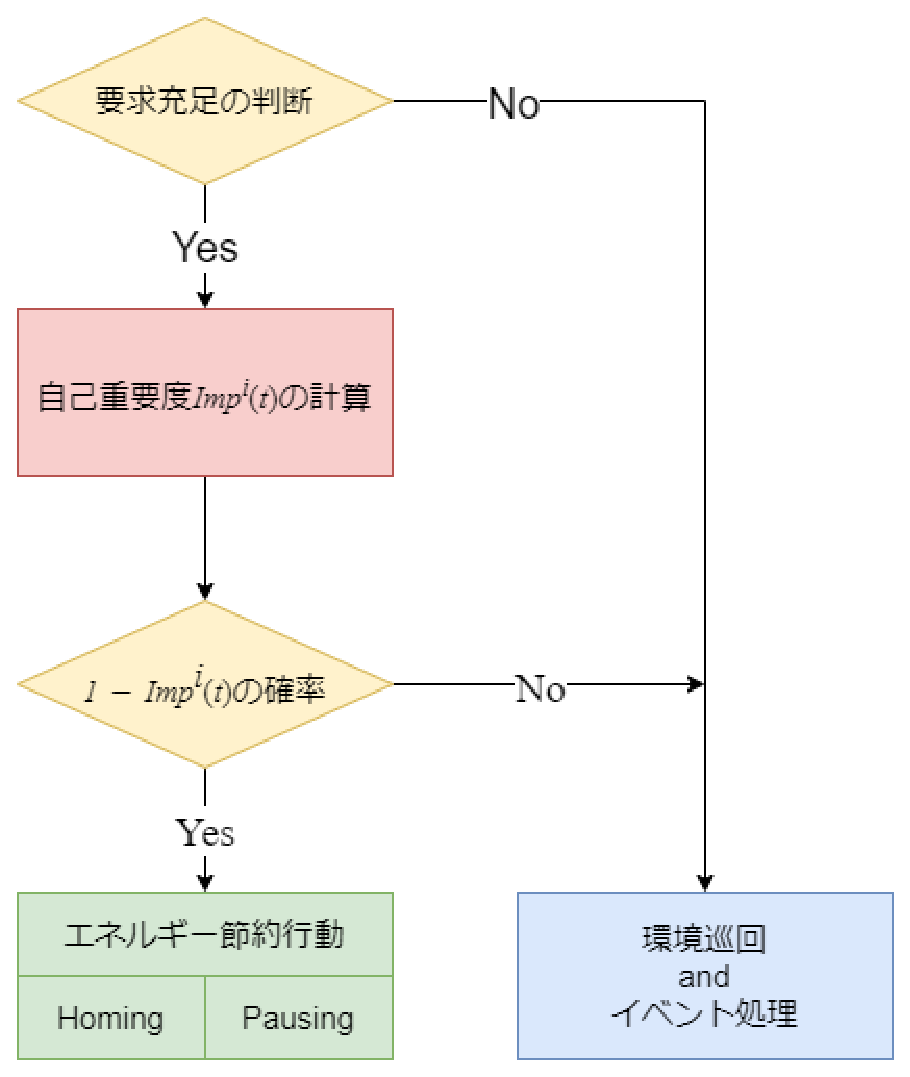
\includegraphics[width=0.6\hsize]{figures/Flowchart.eps}
    \caption{エージェントの行動選択}
    \label{fig:flowchart}
  \end{figure}


  \subsection{AMTDS for energy saving and cleanliness (AMTDS/ESC)}
  AMTDSやAMTDS/LD,AMTDS/EDCでは,イベント残存時間をより小さくすることが求められた.
  しかし,エネルギー消費量も同時に小さくすることができればより有用である.
  つまり,イベント残存時間だけではなく,エネルギー消費を節約することが求められることもある.
  したがって,目標決定戦略を選択するQ学習における報酬の計算方法を,式(\ref{eq:reward_AMTDS})から以下の式に変更し,
  報酬を$r_{t_0,t_0+d_{travel}}$とした,AMTDS for energy saving and cleanliness (AMTDS/ESC) \cite{Wu2019}が提案された.
  %
  \begin{equation}
    r_{t_0,t_0+d_{travel}} = \dfrac{\displaystyle\sum_{t_0+1 \leq t \leq t_0+d_{travel}} L_t(v^i_t)}{d_{travel} \times \displaystyle\sum_{t_0+1 \leq t \leq t_0+d_{travel}} E_t(i)}
  \end{equation}
  %
  これにより,エージェントはより少ないエネルギーでより多くのイベントを処理できる目標決定戦略を決定する.
  なお,目標決定戦略$s_{next}$を$\varepsilon$-Greedy法によって決定するのは,\ref{subsec:AMTDS}と同様である. 
  \par

  AMTDS/ESCではさらに,エネルギー節約行動として,HomingとPausingの2つの行動が導入された.
  図\ref{fig:flowchart}はエージェントにおけるエネルギー節約行動にかかわる行動選択のフローチャートである.
  このフローチャートが示すように,2つの条件が満たされた場合,エージェントはエネルギー節約行動を行う.
  その際に,エージェントは2つのエネルギー節約行動のどちらかを行う.
  エージェントは,不要と思われる行動を排除するために,{\em Homing}または{\em Pausing}の2つのエネルギー節約行動をとる.
  以下でそれぞれの詳細を説明する.

  \subsubsection{要求充足の判断}
  \label{subsec:judge}
  エージェントは,環境の現状を把握し,必要なタスクの品質と比較することで,エネルギー消費を抑える必要がある.
  しかし,どのエージェントも実際の状態を把握することができないため,定期的に推定を行う必要がある.
  そこで,エージェント$i$は,自身が持っている$p^i(v)$を用いて,
  以下の式に従って,時刻$t$における総イベント量$E^i(V_t)$を推定する.
  %
  \begin{equation}
    \label{eq:fulfill}
    E^i(V_t) = \sum_{v \in V} E^i(L_t(v))
  \end{equation}
  %
  その後,要求条件を満たしているのかを判断するために,以下の式を用いている.
  %
  \begin{equation}
    \label{eq:requirement}
    E^i(V_t) \leq D_{req}
  \end{equation}
  %
  この式を満たしていれば$i$は自己重要度評価を行い,満たしていなければ,通常の環境巡回とイベント処理を行う.

  \subsubsection{自己重要度評価}
  エージェントは,\ref{subsec:judge}で述べた方法で要求条件を満たしているかを判断し,
  満たしていた場合,自分の貢献度を評価し,自分のエネルギー節約行動が環境の将来に与える影響を予測する.
  そのために,エージェント$i$の時刻$t$における自己重要度$\SelfAss^i(t)$を導入する.
  これは,$i$が協調タスクのために巡回を継続すべきか,エネルギー節約行動をとって巡回を停止すべきかを決定するための,
  $i$の最近の貢献度合いを表している.
  \par

  $SelfAss^i(t)$を計算するために,以下の3つのパラメータを$\forall i\in\AgentSet$に対して定義する.
  %
  \begin{align}\label{eq:param1}
    U^i_s(t_c) &= \frac{\sum_{t_c-T_s < t \leq t_c} L_t(v^i(t))}{T_s}\\
    U^i_l(t_c) &= \frac{\sum_{t_c-T_l < t \leq t_c} L_t(v^i(t))}{T_l}\label{eq:param2}\\
    U^i_f(t_c) &= \frac{\sum_{t_c < t \leq t_c+T_f} E^i(L_t(v^i(t)))}{T_f},\label{eq:param3}
  \end{align}
  %
  ここで,$t_c$は現在の時刻,$T_s$と$T_l~(0 < T_s < T_l)$は過去の短期・長期の評価期間,$T_f$は将来の評価期間,
  $v^i(t)$は$t$において$i$がいた,またはいる予定のノードを表す.
  直感的には,$U^i_s(t_c)$と$U^i_l(t_c)$は過去に$i$が処理したイベント数を表し,
  $U^i_f(t_c)$は将来$t_c+T_f$までに$i$が処理するであろうイベント数の推定値であるといえる.
  つまり,エージェントは以下の2つを考慮して自己重要度を求めている.
  %
  \begin{enumerate}
    \item[(1)] ある期間における過去の貢献度
    \item[(2)] 重要な領域を発見し,その後の行動で多くのイベントを処理できるか
  \end{enumerate}
  %
  なお,式(\ref{eq:param3})でのみ,$L_t(v^i(t))$の代わりに期待値$E^i(L_t(v^i(t)))$が使用されていることに注意されたい.
  \par

  ここで,自己重要度$\SelfAss^i(t)$ ($0 \leq \SelfAss^i(t) \leq 1$)を次の式のように定義する.
  %
  \begin{equation}\label{Imp}
    \SelfAss^i(t) = 
    \begin{cases}
      \; 0                           & (U^i_l = 0\textrm{ のとき} ) \\
      \; \dfrac{U^i_s + U^i_f}{U^i_l} & (U^i_s + U^i_f \leq U^i_l\textrm{ のとき}) \\
      \; 1                           & (\text{その他})
    \end{cases}\\
  \end{equation}
  %
  その後,$i$は以下の式で求められる確率$P^i(t)$でエネルギー節約行動を選択する.
  %
  \begin{equation}\label{pi(t)}
    P^i(t) = 1 - \SelfAss^i(t)
  \end{equation}
  %
  したがって,自己重要度が低いと,エージェントのエネルギー節約行動が促進される.

  \subsubsection{帰還動作 ({\em Homing})}
  \label{sec:Homing}
  {\em Homing}とは,バッテリ残量にかかわらず,巡回を中止して充電基地に戻ることで,エネルギーを節約する動作のことである.
  エージェント$i$は,充電残量が少なくなり,以下の式を満たしたとき,
  $\HomingCheck$ステップ移動するごとに要求充足度(式(\ref{eq:fulfill}))をチェックする.
  %
  \begin{equation}
    \BatteryLevel^i(t) < \HomingBattery\cdot\BatteryMax
  \end{equation}
  %
  ここで,正の整数$HomingCheck$は{\em Homing}による頻繁な充電基地への帰還を避けるためのパラメータ,
  $\HomingBattery$ ($0 < \HomingBattery < 1$)はバッテリ残量低下を判断するためのパラメータである.
  式(\ref{eq:fulfill})を満たさない場合,$i$は巡回を継続し,
  満たす場合は,確率$P_i(t)$で$i$が現在の$v^i_{tar}$を$v_{charge}$に変更する{\em Homing}を行い,
  充電基地についたら充電を行う.
  また,{\em Homing}中はイベント処理は行うが,要求充足の判定や自己重要度の計算は行わない.
  なお,充電基地から遠い地点を巡回しているエージェントがこのチェックをする前に充電基地に帰還することもありうる.

  \subsubsection{待機動作 ({\em Pausing})}
  \label{sec:Pausing}
  {\em Pausing}とは,充電完了後,エージェントはすぐに巡回を再開せずに,待機する動作のことである.
  エージェント$i$が時刻$t$に充電が完了したとき,要求充足度(式(\ref{eq:fulfill}))をチェックし,
  満たす場合は一定の休止時間$\PausingInt$ステップ充電基地で待機する.
  満たさない場合は,巡回を再開する.
  

  \section{提案手法}
  AMTDS/ESCでは,要求値$\Dreq$とエネルギー節約行動の導入によって,
  品質要求を満たしつつ,エネルギー消費量を削減することができた.
  しかし,{\em Homing}と{\em Pausing}の2つのエネルギー節約行動のうち,どちらか片方しか行うことができなかった.
  また,全てのエージェントが同一の視点で要求充足の判断を行っていたため,
  環境の状態の推定が不十分であり,要求条件を満たす上で不必要な巡回を行っているため,
  エネルギーを余分に消費してしまっている.
  これらの問題を解消するため,本研究では,
  AMTDS for energy saving under the requirement (AMTDS/ER)と,
  AMTDS/EDCに加えたAMTDS for energy saving under the requirement with communications (AMTDS/ERC)
  を提案する.
  以下では,ベースとしている手法との違いに絞って説明する.
  
  \subsection{AMTDS for energy saving under the requirement (AMTDS/ER)}
  この節では,AMTDS/ESCをベースに,エージェントがそれぞれの視点で将来の環境状態を予測する方法を学習し,
  充電基地についた際に,未来の環境状態を予測し,待機時間を動的に決定する手法である,AMTDS/ERについて説明する.
  また,エージェント数を減らす手法についても説明する\red{ここをもっとちゃんと書く}
  

  \subsubsection{未来のイベント量の予測}
  \label{sec:predict}
  AMTDS/ERでは,\ref{sec:changeEnergySaving}で詳しく説明するが,
  {\em Pausing}による待機時間を可変に変更する.
  その際に,未来のイベント量の予測をする必要があるため,その方法について説明する.
  \par

  エージェント$i$は,将来の時刻$t_c+T$における$\forall v\in V$の期待値$E^i(L_{t_c+T}(v))$を,
  以下の式に従って求める.
  %
  \begin{equation}\label{eq:estimation}
    E^i(L_{t_c+T}(v)) = p(v) \times \{(t_c+T)-t^v_{vis}\}
  \end{equation}
  %
  ここで,$T>0$は$i$がどの程度先の未来を推定するかを指定するパラメータである.
  
  \subsubsection{予測の自律的補正学習}
  \ref{sec:predict}で説明した未来のイベント量の予測を行った後,
  エージェント$i$は式(\ref{eq:fulfill})を確認する.
  しかし,この式(\ref{eq:fulfill})は$T$に対して単調増加であるため,
  この推定は,均一な作業量に基づく理想的な場合であり,
  他エージェントによる努力(巡回)は無視されている.
  特に,$i$がエネルギー節約や充電のために巡回を停止していても,
  他エージェントは要求値$\Dreq$を維持しようとする.
  さらに,各エージェントは異なる特徴を持つ場所を訪問するため,
  他エージェントによる努力は,個々の視点によって明らかに異なる.
  したがって,エージェントは,エネルギー節約行動中における他エージェントの
  努力の可能性を学習する必要がある.
  \par

  これを調整するために,学習パラメータ$K^i$を$\forall i\in \AgentSet$に導入する.
  そして,エージェント$i$は,式(\ref{eq:fulfill})の代わりに,
  以下の式を用いて要求条件を満たしているかを判断する.
  % 
  \begin{equation}\label{eq:revised}
    \sum_{v \in V} E^i(L_{t_c+T}(v)) \div K^i \leq \Dreq
  \end{equation} 
  %
  さらに,$K^i$は個々に次の式に従って更新される.
  %
  \begin{equation}
    \begin{cases}
      K^i \gets (1 - \alpha_k)K^i + \alpha_k\dfrac{\Dreq}{E^i(D_t)}
      K^i & (E^i(D_t) \leq \Dreq \textrm{ のとき})\\
      K^i \gets K^i - \left( \dfrac{E^i(D_t)}{\Dreq} - 1 \right) 
      & (E^i(D_t) > \Dreq \textrm{ のとき})
    \end{cases}
    \label{eq:ParameterK}
  \end{equation}
  %
  ここで,$t$におけるイベント量の推定値は$E^i(D_t)=\sum_{v\in V} E^i(L_t(v))$で定義され,
  $\alpha_k>0$は学習率である.
  $K^i$がいつ更新されるかは,\ref{sec:changeEnergySaving}で説明する.


  \begin{algorithm}
    \caption{{\sf PLength}: To decide pausing time-length.}\label{alg:PausingTime}
    \begin{algorithmic}[1]
      \REQUIRE $\PausingInt > 0$, $\PauseTimeFactor=0$, $T_\PauseTimeFactor > 0$
      \WHILE {$\PauseTimeFactor \leq T_\PauseTimeFactor$} 
      \STATE $T\leftarrow (\PauseTimeFactor+1)\cdot\PausingInt$ // $T$ is
      used in Formula~(\ref{eq:revised})
      \IF {Formula~(\ref{eq:revised}) holds}
      \STATE $\PauseTimeFactor \leftarrow \PauseTimeFactor+1$
      \ELSE
      \STATE break
      \ENDIF
      \ENDWHILE
      \STATE // エージェントは待機時間$\PauseTimeFactor\cdot\PausingInt$の{\em Pausing}を行う
      \STATE // もし$\PauseTimeFactor=0$の場合, エージェントは即座に充電基地を出発し,巡回を再開する
      \STATE return $\PauseTimeFactor\cdot\PausingInt$.
    \end{algorithmic}
  \end{algorithm}


  \subsubsection{エネルギー節約行動の修正}
  \label{sec:changeEnergySaving}
  ここでは,より多くのエネルギーを削減するための,
  \ref{sec:Homing}と\ref{sec:Pausing}で説明したエネルギー節約行動の修正点について説明する.
  AMTDS/ESCでは,時刻$t$に充電が完了すると,エージェント$i$が要求条件(式(\ref{eq:fulfill}))を満たす場合,
  $i$は固定の待機時間$PausingInt$ステップ{\em Pausing}を行っていた.
  \par

  しかし,提案手法では,エージェントは推定状態の条件に応じて可変の待機時間をとる.
  $i$は以下で説明する可変長の{\em Pausing}を確率$P_i(t)$で行い,$t$で充電を完了する.
  ただし,例外として,$i$は{\em Homing}によって充電基地$v_{base}$に戻ったときのみ,
  $P_i(t)$を計算せずに,常に可変長の{\em Pausing}を行う.
  これは,{\em Homing}のみでは,エージェントによる,「イベント処理$\rightarrow$充電$\rightarrow$イベント処理$\rightarrow\cdots$」
  のサイクルが短縮しただけで,エネルギー消費量にはあまり影響しない.
  既に環境が要求条件を満たしていて,自分は余力があっても充電基地に戻るべきと判断し{\em Homing}を行っているため,
  {\em Pausing}を行うことは自然であり,エネルギー消費量の減少が見込める.
  \par

  可変長の{\em Pausing}について説明する.
  まず,$i$は待機時間を以下のように決定する(Algorithm~\ref{alg:PausingTime}の\textsf{PLength}参照).
  初期状態では,エージェント$i$は$\PauseTimeFactor=0$,$T=\PausingInt$と設定する.
  時刻$t$にバッテリが満充電になると,$i$は要求充足度をチェックし(式(\ref{eq:revised})),
  満たしていない場合は,$i$は直ちに充電基地から出発し,巡回を再開する.
  つまり,待機時間は0となる.
  満たしている場合は,$\PauseTimeFactor$を1だけインクリメントし,
  $T \leftarrow (\PauseTimeFactor+1)\cdot \PausingInt$とセットする.
  次に,$i$は再び要求度をチェックし,待機時間を決定するか,
  $\PauseTimeFactor=T_\PauseTimeFactor$となるまでこの操作を繰り返す.
  ただし,$T_\PauseTimeFactor$はこの反復の最大値である.
  その後,$i$は$\PauseTimeFactor\cdot\PausingInt$ステップだけ{\em Pausing}を行う.
  エージェントはこの可変長の{\em Pausing}の後は,必ず充電基地を出発する.
  \par

  前述したように,エージェント$i$が{\em Homing}で充電基地に戻る場合,AMTDS/ESCとは異なり,
  充電完了後に必ず可変長の{\em Pausing}を行う.
  この際に,上記のアルゴリズムによって待機時間が0になる可能性もなる.
  以下では,可変長の{\em Pausing}を単に{\em Pausing}と呼ぶ.

  \subsubsection{不要なエージェントの排除}



  




  
  \subsection{AMTDS for energy saving under the requirement with communications (AMTDS/ERC)}
  
  \subsubsection{イベント発生量の予測に使用するノードの範囲の変更}
  
  \subsubsection{補正係数$K^i$の更新方法の変更}
  
  \section{評価実験}

  \subsection{実験環境}
  
  \begin{table}
    \begin{minipage}[t]{.55\textwidth}
      \centering
      \caption{エージェントに関するパラメータ}
      \begin{tabular}{lcr} \\ \hline
        種類 & パラメーター & 値 \\ \hline
        エージェント数 &  |A| & 20 \\ \hline
        バッテリ & $B^i_{max}$ & 900 \\
                   & $B^i_{drain}$ & 1 \\
                   & $k^i_{charge}$ & 3 \\ \hline
        経路生成戦略 & $d_{myopia}$ & 10 \\
                     & $k_{att}$ & 1.0 \\
                     & $k_{rover}$ & 1.2 \\ \hline
      \end{tabular}
      \label{tb:1}
    \end{minipage}
    %
    \hfill
    %
    \begin{minipage}[t]{.55\textwidth}
      \centering
      \caption{目標決定戦略のパラメーター}
      \begin{tabular}{lcrr} \\ \hline
        目標決定戦略 & パラメーター & 値 \\ \hline
        PGS & $N_g$ & 5 \\ \hline
        PI & $N_i$ & 5 \\ \hline
        BNPS & $\alpha$ & 0.1 \\
             & $d_{rad}$ & 15 \\ \hline
        AMTDS & $\alpha$ & 0.1 \\
              & $\varepsilon$ & 0.05 \\ \hline
        AMTDS/LD & $\beta$ & 0.1 \\ \hline 
      \end{tabular}
      \label{tb:2}
    \end{minipage}
    %
    \vskip\baselineskip
    %
    \begin{minipage}[t]{.55\textwidth}
      \centering
      \caption{エネルギー節約行動に関するパラメーター}
      \begin{tabular}{lcrr} \\ \hline
        種類 & パラメーター & 値 \\ \hline
        自己重要度評価 & $T_s$ & 20 \\
                       & $T_l$ & 50 \\
                       & $T_f$ & 10 \\ \hline
        Homing & $T_{check}$ & 100 \\
               & $k_{homing}$ & $1/3$ \\ \hline
        Pausing & $T_{basic}$ & 100 \\ \hline  
        AMTDS/ERL & $T_{hp}$ & 500,000 \\ \hline       
      \end{tabular}
      \label{tb:3}
    \end{minipage}
  \end{table}

  \subsection{AMTDS/ERについての実験結果}
  \label{result_ER}
  
  \subsubsection{実験1: 性能評価}
  \label{ex:ER1}
  
  \subsubsection{実験2: 環境の変化による性能の違い}
  \label{ex:ER2}

  \subsubsection{実験3: エージェント数減少による性能の変化}

  \subsubsection{実験4: $\Dreq$の変化による性能の変化}

  \subsection{AMTDS/ERCについての実験結果}
  \label{result_ERC}
  
  \subsubsection{実験5: 性能評価}
  \label{ex:ERC1}
  
  \subsubsection{実験6: 環境の変化による性能の違い}
  \label{ex:ERC2}  
  
  \subsubsection{実験7: エージェント数減少による性能の変化}

  \subsubsection{実験8: $K^i$の降順にエージェント数を減少させたときの性能の変化}

  \section{結論}

  \clearpage
  \bibliographystyle{junsrt}
  \bibliography{ref}

\end{document}